\begin{frame}{What is {\it Scheduling}?}
  \vfill
  \begin{block}{Larousse}
    {\bf \color{bleuLAAS} Scheduling: }organization, methodical arrangement of the different
    element of a set, of the  different phases of a fabrication.
  \end{block}
  \vfill
  \begin{block}{Cambridge}
    {\bf  \color{bleuLAAS}  Scheduling: }the job or activity of planning the times at which particular tasks will be done or events will happen.
  \end{block}
  \vfill  
  \begin{block}{Wikipedia}
    A {\bf  \color{bleuLAAS}  scheduling} problem consists in organizing the realization of
    tasks through time, given time constraints (setup time, precedence)
    and constraints on the availability of required resources.
  \end{block}
  \vfill
\end{frame}

\begin{frame}{What is {\it Scheduling}?}
\vspace{0.3cm}
  \begin{block}{My thesis}
    The {\bf  \color{bleuLAAS} scheduling} theory aims at computing {\bf activities execution
      start/end times} subject to a certain number of {\bf
      constraints} in order to optimize an {\bf objective}.    
  \end{block}
  \vspace{0.6cm}
  \begin{description}
  \item[activities :]  courses, landing/taking off, step in a
    construction project... 
    \vspace{0.2cm}
  \item[constraints :]
    \begin{itemize}
    \item temporal $\rightarrow$ deadline, precedence, setup...
    \item resource $\rightarrow$ availability, nature... 
    \end{itemize}
    \vspace{0.2cm}
  \item[objective :] resource consumption, total cost, makespan,
    tardiness... 
    \vspace{0.2cm}
  \end{description}
\end{frame}

\begin{frame}{Application example: Timetable}
  
  {\usebeamercolor[fg]{item} activities: } is a set of courses\\[0.2cm]
          {\usebeamercolor[fg]{item} temporal constraints: } Precedence relationship: lecture before
            exercise, Analysis 1 before Analysis 2...\\[0.2cm]

         {\usebeamercolor[fg]{item} resource constraints: }rooms, teachers, additional material...\\[0.2cm]

         \vfill
      \begin{center}
      \includegraphics[scale=0.25]{figures/timetable.png}
    \end{center}
\vspace{-0.5cm}    
\end{frame}


\begin{frame}{Resource and activity characteristics}
    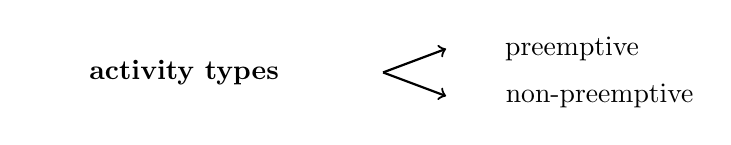
\begin{tikzpicture}\tikzstyle{every node} = [align=center]
      \node at (0,0) {\bf \phantom{ain} activity types \phantom{ons}};

      \draw[thick,->] (2.5,0) -- (3.3,0.3);
      \draw[thick,->] (2.5,0) -- (3.3,-0.3);

      \node at (4.9,0.3)  {preemptive};
      \node at (5.25,-0.3) {non-preemptive};
    \end{tikzpicture}
\vfill
  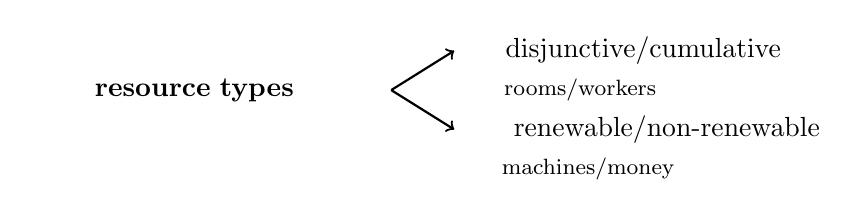
\begin{tikzpicture}\tikzstyle{every node} = [align=center]
    \node[text width=4cm] at (0,0) { \bf resource types };

    \draw[thick,->] (2.5,0) -- (3.3,0.5);
    \draw[thick,->] (2.5,0) -- (3.3,-0.5);

    \draw[white] (0,0);
    \node at (5.7,0.5)  {disjunctive/cumulative};
    \node at (4.9,0)  {\footnotesize rooms/workers};
    \node at (6,-0.5) {renewable/non-renewable};
    \node at (5,-1)  {\footnotesize machines/money};
  \end{tikzpicture}
  \vfill
  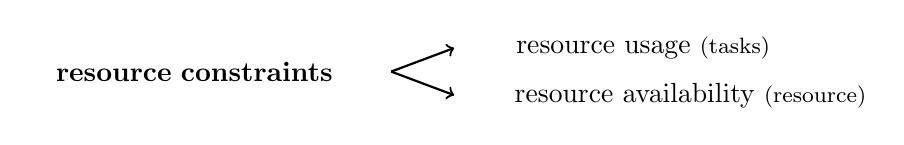
\begin{tikzpicture}\tikzstyle{every node} = [align=center]
    \node at (0,0) {};
    \node[text width=4cm] at (0,0) { \bf resource constraints };

    \draw[thick,->] (2.5,0) -- (3.3,0.3);
    \draw[thick,->] (2.5,0) -- (3.3,-0.3);

    \node at (5.7,0.3)  {resource usage {\footnotesize (tasks)}};
    \node at (6.3,-0.3) {resource availability {\footnotesize (resource)}};
  \end{tikzpicture}
  \vspace{-1cm}
\end{frame}

\begin{frame}
  \frametitle{The Cumulative Scheduling Problem} 
\vfill
 \textbf{Inputs : }
\vfill
  \begin{itemize}
  \item a set ${\cal A}=\{1,\dots ,n\}$ of non-preemptive tasks
      \vfill
    \item a cumulative and renewable resource available in quantity $B$
      \vfill
    \item<2-> for each task:
      \begin{columns}
        \hfill
        \begin{column}{0.5\linewidth}
          \vspace{-0.5cm}
          \begin{itemize}
          \item<2-> \footnotesize  a processing time $p_i$
            \vfill
          \item<3-> \footnotesize a resource consumption $b_i$ 
            \vfill
          \item<4-> \footnotesize a release date $r_i$ and a deadline $d_i$ 
            \vfill
          \end{itemize}
        \end{column}
        \hfill
        \begin{column}{0.4\linewidth}
          \centering
          \vspace{0.8cm}
          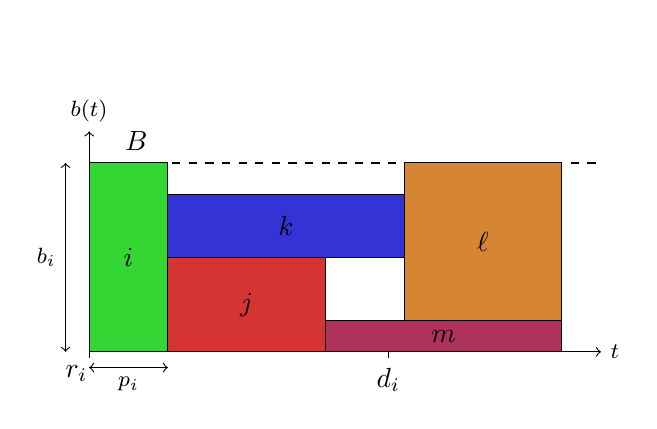
\begin{tikzpicture}
  [yscale=0.4]
  \node at (0,10) {};

  \node[label={[shift={(-0.4,-0.5)}]}] (O) at (0,0) {};
  \draw[fill=red!80!black!80] (1,0) rectangle (3,3)   node[midway] {$j$};
  \draw[dashed,thick] (0,6)   -- (6.5,6);
  \node at (0.6,6.7)  {$B$};
    \draw[<->] (0,-0.5) -- (1,-0.5) node[midway,below] {\footnotesize $p_i$};
    \draw[<->] (-0.3,0) -- (-0.3,6) node[midway,left] {\footnotesize $b_{i}$};
  
  \draw (0,0) -- (0,-0.2) node[below=0.2cm,left=-0.1cm] {$r_i$};
  \draw (3.8,0) -- (3.8,-0.2) node[below] {$d_i$};
  
  \draw[fill=green!80!black!80] (0,0) rectangle (1,6)   node[midway] {$i$};
  \draw[fill=blue!80!black!80] (1,3) rectangle (4,5)   node[midway] {$k$};
  \draw[fill=orange!80!black!80] (4,1) rectangle (6,6)   node[midway] {$\ell$};
  \draw[fill=purple!80!black!80] (3,0) rectangle (6,1)   node[midway] {$m$};
  \draw[->] (O.center) -- (0,7) node[above] {\footnotesize $b(t)$};
  \draw[->] (O.center) -- (6.5,0) node[right] {\footnotesize $t$};


\end{tikzpicture}

      \end{column} 
    \end{columns}
  \end{itemize}
\vfill
\only<5->{
\textbf{Application : }
\vfill
  \begin{itemize}
  \item electricity consumption cannot exceed a certain level.
  \end{itemize}}
\end{frame}


\begin{frame}{Solution methods for the CuSP}
  
\end{frame}

\begin{frame}
  \frametitle{Limitations}
 \vspace{0.5cm}
  \begin{itemize}
  \item Several scheduling problems deal with resource constraints
    \vfill
  \item {Limitation} : fixed duration and resource consumption
    \vfill
  \item<4-> But, in practice, it is not always the case\\
   \end{itemize}
  \vspace{1cm}
  \begin{columns}
\hfill
    \begin{column}{0.45\linewidth}
      \centering
      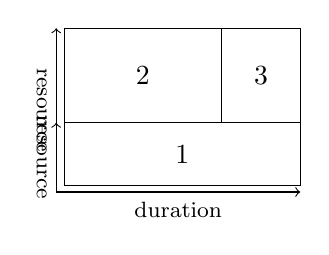
\begin{tikzpicture}
        [xscale=0.5,yscale=0.4]
        \node (O) at (0,0) {};
        \onslide<2>{
          \draw (0,0) rectangle (6,2);
          \draw[->](-0.2,-0.2) -- (-0.2,2) node[midway,below,rotate=-90] {\footnotesize resource};}
        \onslide<3->{
          \draw (0,0) rectangle (6,2) node[midway] {$1$};
          \draw (0,2) rectangle (4,5) node[midway] {$2$};
          \draw (4,5) rectangle (6,2) node[midway] {$3$};
          \draw[->](-0.2,-0.2) -- (-0.2,5) node[midway,below,rotate=-90] {\footnotesize resource};
        }
        \onslide<2->{
        \draw[->] (-0.2,-0.2) -- (6,-0.2) node[midway,below] {\footnotesize duration};}
      \end{tikzpicture}
    \end{column}
    \hfill
    \begin{column}{0.45\linewidth}
      \centering
      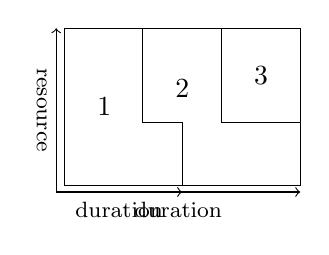
\begin{tikzpicture}
        [xscale=0.5,yscale=0.4]
        \node (O) at (0,0) {};
        \onslide<5> {
          \draw[->] (-0.2,-0.2) -- (3,-0.2) node[midway,below] {\footnotesize duration};}
        \onslide<6->{
          \path[draw] (0,0) -- (0,5) -- (2,5) -- (2,2) -- (3,2)  node[above=0.2cm] {$2$} -- (3,0)-- cycle;
          \path[draw] (2,5) -- (4,5) -- (4,2) -- (6,2) -- (6,0) --(3,0);
          \draw (4,2) rectangle (6,5) node[midway] {$3$};
          \draw[->] (-0.2,-0.2) -- (6,-0.2) node[midway,below] {\footnotesize duration};
        }
        \onslide<5-> {
          \path[draw] (0,0) node[above=1cm,right=0.3cm] {$1$}-- (0,5) -- (2,5) -- (2,2) -- (3,2) -- (3,0)-- cycle;
          \draw[->](-0.2,-0.2) -- (-0.2,5) node[midway,below,rotate=-90] {\footnotesize resource};}
      \end{tikzpicture}
    \end{column}
\hfill
  \end{columns}
\end{frame}


\begin{frame}
  \frametitle{Motivating Problem: Melting metal in a foundry}
  {\small \it \color{gray!50!black!50} [Artigues et al., 2013]}
  \vfill
  \begin{columns}
    \begin{column}{0.5\linewidth}
      \begin{itemize}
      \item a set of melting jobs
        \vspace{0.4cm}
      \item melting operation has variable duration\\
        {\small (depending of the power given + may vary over time)}
         \vspace{0.4cm}
      \end{itemize}     
    \end{column}
    \hfill 
    \begin{column}{0.4\linewidth}
      \includegraphics[width=0.8\linewidth]{figures/induction.jpg}
    \end{column}
  \end{columns}
  \vfill
  \begin{itemize}
  \item upper and lower bound on the power given \\
    {\small(operational and physical consideration)}
    \vspace{0.4cm}
  \item electrical power limitation\\
    {\small(electrical overrun cost)}
  \end{itemize}
\end{frame}


\begin{frame}{Literature review}
  
\end{frame}

\begin{frame}{The Energy Scheduling Problem (EnSP)}
  
\end{frame}

\begin{frame}{Solution Method for the EnSP and limitations}
  
\end{frame}

\begin{frame}{The Continuous Energy Constrained Scheduling Problem (CECSP)}
   Generalization of the CuSP
  \begin{itemize}
    \vfill
  \item Duration $p_i$ $\leftrightarrow$ required energy amount $W_i$
    \vfill
  \item Fixed resource consumption $b_i$ $\leftrightarrow$ variable resource consumption (within an interval)
    \vfill  
  \item Task can take any shape bounded by:
    \begin{itemize}
    \item<2-> its time-window
    \item<3-> a maximal and minimal resource consumption
    \item<4-> energy amount that has to be received by the task
    \end{itemize}
    \vfill
  \end{itemize}
  \begin{overlayarea}{\textwidth}{3cm}
    \only<1-4> {
      \vfill
      \begin{columns}
        \begin{column}{0.45\linewidth}
          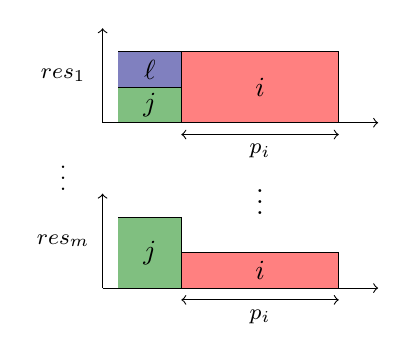
\begin{tikzpicture}
  [yscale=0.3]
  \node[label={[shift={(-0.4,-0.5)}]}] (O) at (0,0) {};
  \draw[fill=red!50] (1,0) rectangle (3,3)   node[midway] {$i$};
  
  \onslide<2-3>{
    \draw[<->] (1,-0.5) -- (3,-0.5) node[midway,below] {\footnotesize $p_i$};
  }
  \onslide<3>{
    \draw[<->] (0.8,0) -- (0.8,3) node[midway,left] {\footnotesize $b_{i1}$};
  }
  
  \draw[->] (O.center) -- (0,4);
  \draw[->] (O.center) -- (3.5,0);


  \onslide<3->{
  \node at (2,-3) {$\vdots$};

  \draw[fill=red!50] (1,-7)rectangle (3,-5.5) node[midway] {$i$};
  
  \onslide<3>{
    \draw[<->] (1,-7.5) -- (3,-7.5) node[midway,below] {\footnotesize $p_i$};
  }
  \onslide<3>{
    \draw[<->] (0.8,-7) -- (0.8,-5.5) node[midway,left]
    {\footnotesize $b_{im}$};
  }
  
  \node at (-0.5,2) {\footnotesize $res_1$};
  \node at (-0.5,-5) {\footnotesize $res_m$};
  \node at (-0.5,-2) {\footnotesize $\vdots$};

  \draw[->] (0,-7) -- (0,-3);
  \draw[->] (0,-7) -- (3.5,-7);
}
\onslide<4->{
  \fill[color=green!50!black!50] (0.2,0) rectangle (1,1.5);
  \draw (0.2,0) -- (1,0) -- (1,1.5) -- (0.2,1.5) ;
  \path (0.2,0.75) -- (1,0.75) node[midway] {$j$};

  \fill[color=blue!50!black!50] (0.2,1.5) rectangle (1,3);
  \draw (0.2,1.5) -- (1,1.5) -- (1,3) -- (0.2,3) ;
  \path (0.2,2.25) -- (1,2.25) node[midway] {$\ell$};


  \fill[color=green!50!black!50] (0.2,-7) rectangle (1,-4);
  \draw (0.2,-7) -- (1,-7) -- (1,-4) -- (0.2,-4) ;
  \path (0.2,-5.5) -- (1,-5.5) node[midway] {$j$};
}
\end{tikzpicture}

        \end{column}
        \begin{column}{0.45\linewidth}
          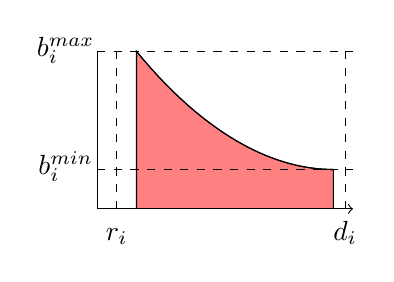
\begin{tikzpicture}
  [scale=0.5]
  \node (O) at (0,0) {};
  \onslide<4->{  
    \path[draw, fill=red!50] (1,0) -- (1,4) parabola [bend at end] (6,1) -- (6,0); 
  }
  \onslide<2->{
    \node[label={[shift={(0,-0.7)}]$r_i$}]  at (0.5,0) {};
    \node[label={[shift={(0,-0.7)}]$d_i$}]  at (6.3,0) {};
    \draw[dashed] (0.5,0) -- (0.5,4);
    \draw[dashed] (6.3,0) -- (6.3,4);
  }
  \onslide<3->{
    \node[label={[shift={(-0.4,-0.4)}]$b_i^{min}$}]  at (0,1) {};
    \node[label={[shift={(-0.4,-0.4)}]$b_i^{max}$}]  at (0,4) {};
    \draw[dashed] (0,1) -- (6.5,1);
    \draw[dashed] (0,4) -- (6.5,4);}
  
  
  \draw (O.center) -- (0,4);
  \draw[->] (O.center) -- (6.5,0);
  
  \draw (1,4) -- (1,0);
  
  
  \path[draw] (1,4) parabola [bend at end] (6,1); 
  
  \draw (6,1) -- (6,0);
\end{tikzpicture}

        \end{column}
      \end{columns}
      \vfill}
    \only<5>{
      \vfill
      \begin{itemize}
      \item Modeled with a continuous resource
      \end{itemize}
      \vfill 
      $\Rightarrow$ \textbf{Continuous Energy-Constrained Scheduling Problem (CECSP) {\scriptsize \color{gray!50!black!50} \it [Artigues \& Lopez, JoS, 2015]}}
      \vfill}
  \end{overlayarea}
\end{frame}

\begin{frame}
  \frametitle{Problem statements}
  \vfill
  Input:\\
  \begin{itemize}
  \item $A=\{1,\hdots,n\}$ a set of non-preemptive tasks
  \item a continuous, cumulative and renewable resource of capacity  $B$
  \end{itemize}
  \vfill
  \onslide<2->{
    Output: A scheduling, i.e. a start time $st_i$, an end time $ft_i$ and a resource allocation function $b_i(t)$, such that:
  }
  \begin{overlayarea}{\linewidth}{1cm}
    \only<3>{\[r_i\le st_i\le ft_i \le d_i\]}
    \only<4>{\[\bmin \le b_i(t) \le \bmax \quad \forall t \in \inter[st_i][ft_i]\]}
    \only<5>{\[b_i(t)=0\quad \forall t \not\in \inter[st_i][ft_i]\]}
    \only<6>{\[\int_{st_i}^{ft_i}b_i(t)dt=W_i\]}
    \only<7>{\[\sum_{i\in A}b_i(t) \le B\]} 
  \end{overlayarea}
  \onslide<2->{
    \begin{center}
      \input{/home/mnattaf/Documents/input_latex/form2_bi.tex}
    \end{center}}
\end{frame}

\begin{frame}{Example for the CECSP$_{id}$}
  
\end{frame}

\begin{frame}{Solution Method for the CECSP$_{id}$ and limitations}
  
\end{frame}

\begin{frame}{Approximation of efficiency functions with the CECSP$_{id}$}
  
\end{frame}

\begin{frame}{The CECSP with linear efficiency functions (CECSP$_{lin}$)}
    \vfill
  In most cases, resource $\neq$ energy
  \vfill
  \begin{block}{Example of the foundry} 
    Metal needs heat and the resource is electricity
  \end{block}
  \vfill
  Important issue if you handle different energy types
  \vfill
  $\Rightarrow$ We need a conversion function $f_i$
  \vfill
  \[W_i=\int_{st_i}^{ft_i}b_i(t)dt \rightarrow W_i=\int_{st_i}^{ft_i}f_i(b_i(t))dt\]
  \vfill
  Here, $f_i(b)$ is non-decreasing, continuous and linear: $f_i(b)=a_i*b+c_i$ 
  \vfill
\end{frame}

\begin{frame}{Example for the CECSP$_{lin}$}
  
\end{frame}

\begin{frame}{Approximation of efficiency functions with the CECSP$_{lin}$}
  
\end{frame}

\begin{frame}{The CECSP with concave piecewise linear efficiency functions (CECSP$_{cpwl}$)}
  
\end{frame}

\begin{frame}
  \frametitle{Solution methods}
  \vfill
  \begin{description}[Properties]
  \item[Properties] {\small
      \begin{itemize}
    \item study of the structural properties of the problem:
      {\footnotesize Dominance rules, complexity analysis, polynomial cases...}
    \end{itemize}}
\vfill
  \item[CP] {\small
    \begin{itemize}
    \item satisfiability test (checker): {\footnotesize Energetic
        reasoning, Flow based checker...}
    \item filtering algorithm: {\footnotesize Energetic reasoning, time-table
      disjunctive reasoning...}
    \item discrete model
    \end{itemize}}
\vfill
  \item[MILP] {\small
      \begin{itemize}
    \item MILP model: {\footnotesize time-indexed, event-based...}
    \item valid inequalities
    \item polyhedral results
    \end{itemize}}
\vfill
  \item[Hybrid] {\small
      \begin{itemize}
    \item ``CP-like branching'' + MILP 
    \item valid inequalities deduced from ER
    \end{itemize}}
  \end{description}
\end{frame}

\setcounter{tocdepth}{20}
\begin{frame}{Overview}
\tableofcontents[hideothersubsections,subsubsectionstyle={show/show/show/show}]
\end{frame}
